\chapter{Analyse et spécification des besoins}
\label{ch:besoins}
\startcontents[chapters]
\chapterplan

\section{Introduction}

Ce chapitre précise ce que la plateforme doit faire, pour qui et selon quelles exigences de qualité. Nous identifions d'abord les acteurs et la répartition de leurs droits, puis nous formulons les besoins fonctionnels et non fonctionnels. Nous les synthétisons dans un diagramme de cas d'utilisation global. Nous présentons ensuite le pilotage du projet : le backlog produit, l'équipe et la planification des sprints. Nous terminons par le diagramme de classes d'analyse, qui décrit les principales notions manipulées par la plateforme.

\section{Identification des acteurs}

Quatre acteurs humains et un acteur système interagissent avec SEPAPaie. Le tableau~\ref{tab:acteurs} précise leur rôle.

\begin{table}[H]
\centering
\small
\renewcommand{\arraystretch}{1.25}
\tablestyle
\begin{tabularx}{\textwidth}{|>{\raggedright\arraybackslash}p{3cm}|Y|}
\hline
\rowcolor{appMarine}\entete{Acteur} & \entete{Rôle et responsabilités} \\
\hline
Expert RH & Prépare les virements de masse : saisit les fiches de paie, génère le fichier SEPA, le contrôle et le soumet au Manager. Il ne travaille que sur les sociétés qui lui sont affectées. \\
\hline
Manager & Approuve les fiches de paie, valide ou rejette les fichiers soumis, affecte les sociétés aux Experts RH et traite les anomalies. \\
\hline
Administrateur & Gère les comptes, les sociétés débitrices et les schémas XSD, consulte le journal d'audit et supervise le module d'IA. Il suit l'activité par des vues globales, sans accéder aux données individuelles de paie. \\
\hline
Visiteur & Demande la création d'un compte ; celui-ci n'est actif qu'après approbation de l'administrateur. \\
\hline
Module d'IA & Acteur système : attribue un niveau de risque aux fiches de paie et explique ses signalements. \\
\hline
\end{tabularx}
\caption{Acteurs de la plateforme}
\label{tab:acteurs}
\end{table}

La banque, destinataire final du fichier, reste en dehors du périmètre de la plateforme : SEPAPaie prépare et valide le fichier, mais ne le transmet pas.

\subsection{Principe de séparation des rôles}

La répartition des droits repose sur deux principes. Le premier est celui des \textbf{quatre yeux} : la personne qui prépare et soumet un fichier ne peut pas le valider, cette décision revenant au Manager. Le second est celui du \textbf{moindre privilège} : chaque profil n'accède qu'aux fonctions nécessaires à sa mission. En particulier, l'administrateur gère la plateforme sans consulter les données de paie des salariés, et l'Expert RH est limité aux sociétés qui lui sont affectées. Le tableau~\ref{tab:droits} résume ces droits.

\begin{table}[H]
\centering
\small
\renewcommand{\arraystretch}{1.2}
\tablestyle
\begin{tabularx}{\textwidth}{|>{\raggedright\arraybackslash}X|>{\centering\arraybackslash}p{1.9cm}|>{\centering\arraybackslash}p{1.9cm}|>{\centering\arraybackslash}p{1.9cm}|}
\hline
\rowcolor{appMarine}\entete{Fonction} & \entete{Admin.} & \entete{Manager} & \entete{Expert RH} \\
\hline
Gérer les utilisateurs et les sociétés débitrices & $\checkmark$ & -- & -- \\
\hline
Consulter le journal d'audit & $\checkmark$ & -- & -- \\
\hline
Superviser et réentraîner le module d'IA & $\checkmark$ & -- & -- \\
\hline
Gérer les schémas XSD & $\checkmark$ & $\checkmark$ & -- \\
\hline
Affecter les sociétés aux Experts RH & -- & $\checkmark$ & -- \\
\hline
Saisir et supprimer les fiches de paie & -- & -- & $\checkmark$ \\
\hline
Approuver les fiches de paie & -- & $\checkmark$ & -- \\
\hline
Générer, contrôler et soumettre un fichier SEPA & -- & -- & $\checkmark$ \\
\hline
Valider ou rejeter un fichier SEPA & -- & $\checkmark$ & -- \\
\hline
Traiter les anomalies & -- & $\checkmark$ & $\checkmark$ \\
\hline
Consulter le détail d'un fichier (XML, salariés) & -- & $\checkmark$ & $\checkmark$ \\
\hline
Consulter l'historique des fichiers & $\checkmark$\textsuperscript{1} & $\checkmark$ & $\checkmark$ \\
\hline
Consulter le tableau de bord et les KPI & $\checkmark$\textsuperscript{2} & $\checkmark$ & $\checkmark$\textsuperscript{3} \\
\hline
\end{tabularx}
\caption{Droits par profil}
\label{tab:droits}
\par\smallskip
{\footnotesize\raggedright \textsuperscript{1}~Supervision en lecture seule, sans données individuelles. \textsuperscript{2}~Vue globale agrégée. \textsuperscript{3}~Limité aux sociétés affectées, montants masqués.\par}
\end{table}

\section{Besoins fonctionnels}

Les besoins fonctionnels sont regroupés en sept modules, présentés dans le tableau~\ref{tab:besoins-fonctionnels}.

\begin{table}[H]
\centering
\small
\renewcommand{\arraystretch}{1.25}
\tablestyle
\begin{tabularx}{\textwidth}{|>{\raggedright\arraybackslash}p{3.4cm}|Y|}
\hline
\rowcolor{appMarine}\entete{Module} & \entete{Besoins fonctionnels} \\
\hline
Comptes et accès & Créer un compte avec photo du visage ; faire approuver ou rejeter les inscriptions par l'administrateur ; s'authentifier par mot de passe suivi d'un code à usage unique, ou par reconnaissance faciale ; gérer les utilisateurs et leurs rôles. \\
\hline
Référentiels & Gérer les sociétés débitrices (code, nom, IBAN, BIC) ; affecter les sociétés aux Experts RH ; importer, modifier et supprimer les schémas XSD. \\
\hline
Fiches de paie & Saisir des fiches de paie en les rattachant à une société, et les supprimer ; les faire approuver par le Manager. \\
\hline
Virement de masse & Sélectionner des fiches par société et par période ; générer un fichier \texttt{pain.001} selon le schéma choisi ; le valider contre le XSD et en prévisualiser le contenu ; soumettre le fichier ; le valider ou le rejeter avec un motif ; conserver chaque fichier de façon immuable dans un historique. \\
\hline
Détection des anomalies & Contrôler les IBAN, les BIC, les montants et les doublons ; détecter par IA les montants atypiques ; associer à chaque anomalie une explication et une recommandation ; suivre son traitement (ouverte, corrigée, ignorée). \\
\hline
Pilotage & Fournir à chaque profil un tableau de bord de ce qu'il doit traiter et des indicateurs de suivi (taux d'approbation, taux d'erreur, conformité XSD, anomalies, apport de l'IA). \\
\hline
Traçabilité & Enregistrer les actions sensibles (connexion, import de schéma, génération, soumission, validation, rejet, affectation) avec leur auteur, leur date et leur résultat. \\
\hline
\end{tabularx}
\caption{Besoins fonctionnels par module}
\label{tab:besoins-fonctionnels}
\end{table}

\section{Besoins non fonctionnels}

Les besoins non fonctionnels expriment la qualité attendue de la plateforme :
\begin{itemize}
    \item \textbf{Sécurité} : authentification par jeton, mots de passe et codes à usage unique conservés sous forme hachée, contrôle des droits côté serveur pour chaque action, lecture des fichiers XML protégée contre les entités externes (attaque XXE) ;
    \item \textbf{Confidentialité} : IBAN masqués à l'affichage, accès de l'administrateur limité à des données agrégées, accès de l'Expert RH limité à ses sociétés ;
    \item \textbf{Traçabilité} : toute action sensible est journalisée et non modifiable depuis l'interface ;
    \item \textbf{Fiabilité} : un fichier non conforme à son schéma ne peut être ni soumis ni téléchargé, et son téléchargement ultérieur restitue exactement le contenu initial ;
    \item \textbf{Résilience de l'IA} : l'indisponibilité ou la désactivation du module d'IA ne doit jamais interrompre le contrôle d'un fichier ; l'IA reste une aide à la décision ;
    \item \textbf{Explicabilité} : tout signalement de l'IA s'accompagne d'une explication lisible et d'une recommandation ;
    \item \textbf{Performance} : temps de réponse compatibles avec un usage interactif, listes paginées ;
    \item \textbf{Ergonomie} : interface claire, adaptée à chaque profil, avec des libellés et des statuts sans ambiguïté ;
    \item \textbf{Portabilité et maintenabilité} : déploiement reproductible par conteneurs, code organisé en couches et couvert par des tests automatisés.
\end{itemize}

\section{Diagramme de cas d'utilisation global}

La figure~\ref{fig:uc-global} présente les cas d'utilisation de la plateforme. Conformément aux règles de modélisation UML, chaque cas d'utilisation représente une action atomique bien délimitée : la validation et le rejet d'un fichier, le contrôle et la génération, la gestion des utilisateurs et la validation des inscriptions, ainsi que la consultation du tableau de bord et des indicateurs KPI constituent des cas distincts. Les cas d'utilisation sont de plus regroupés par périmètre de responsabilité (Périmètre Administrateur, Périmètre Manager, Périmètre Expert RH, et Fonctions communes), reflétant le cloisonnement des rôles. Les trois profils héritent du rôle d'utilisateur authentifié, ce qui factorise les fonctions communes : s'authentifier, consulter l'historique des fichiers, le tableau de bord et les indicateurs. Le cas \og Contrôler un virement de masse\fg{} inclut l'analyse des montants par le module d'IA, acteur système.

\begin{figure}[H]
    \centering
    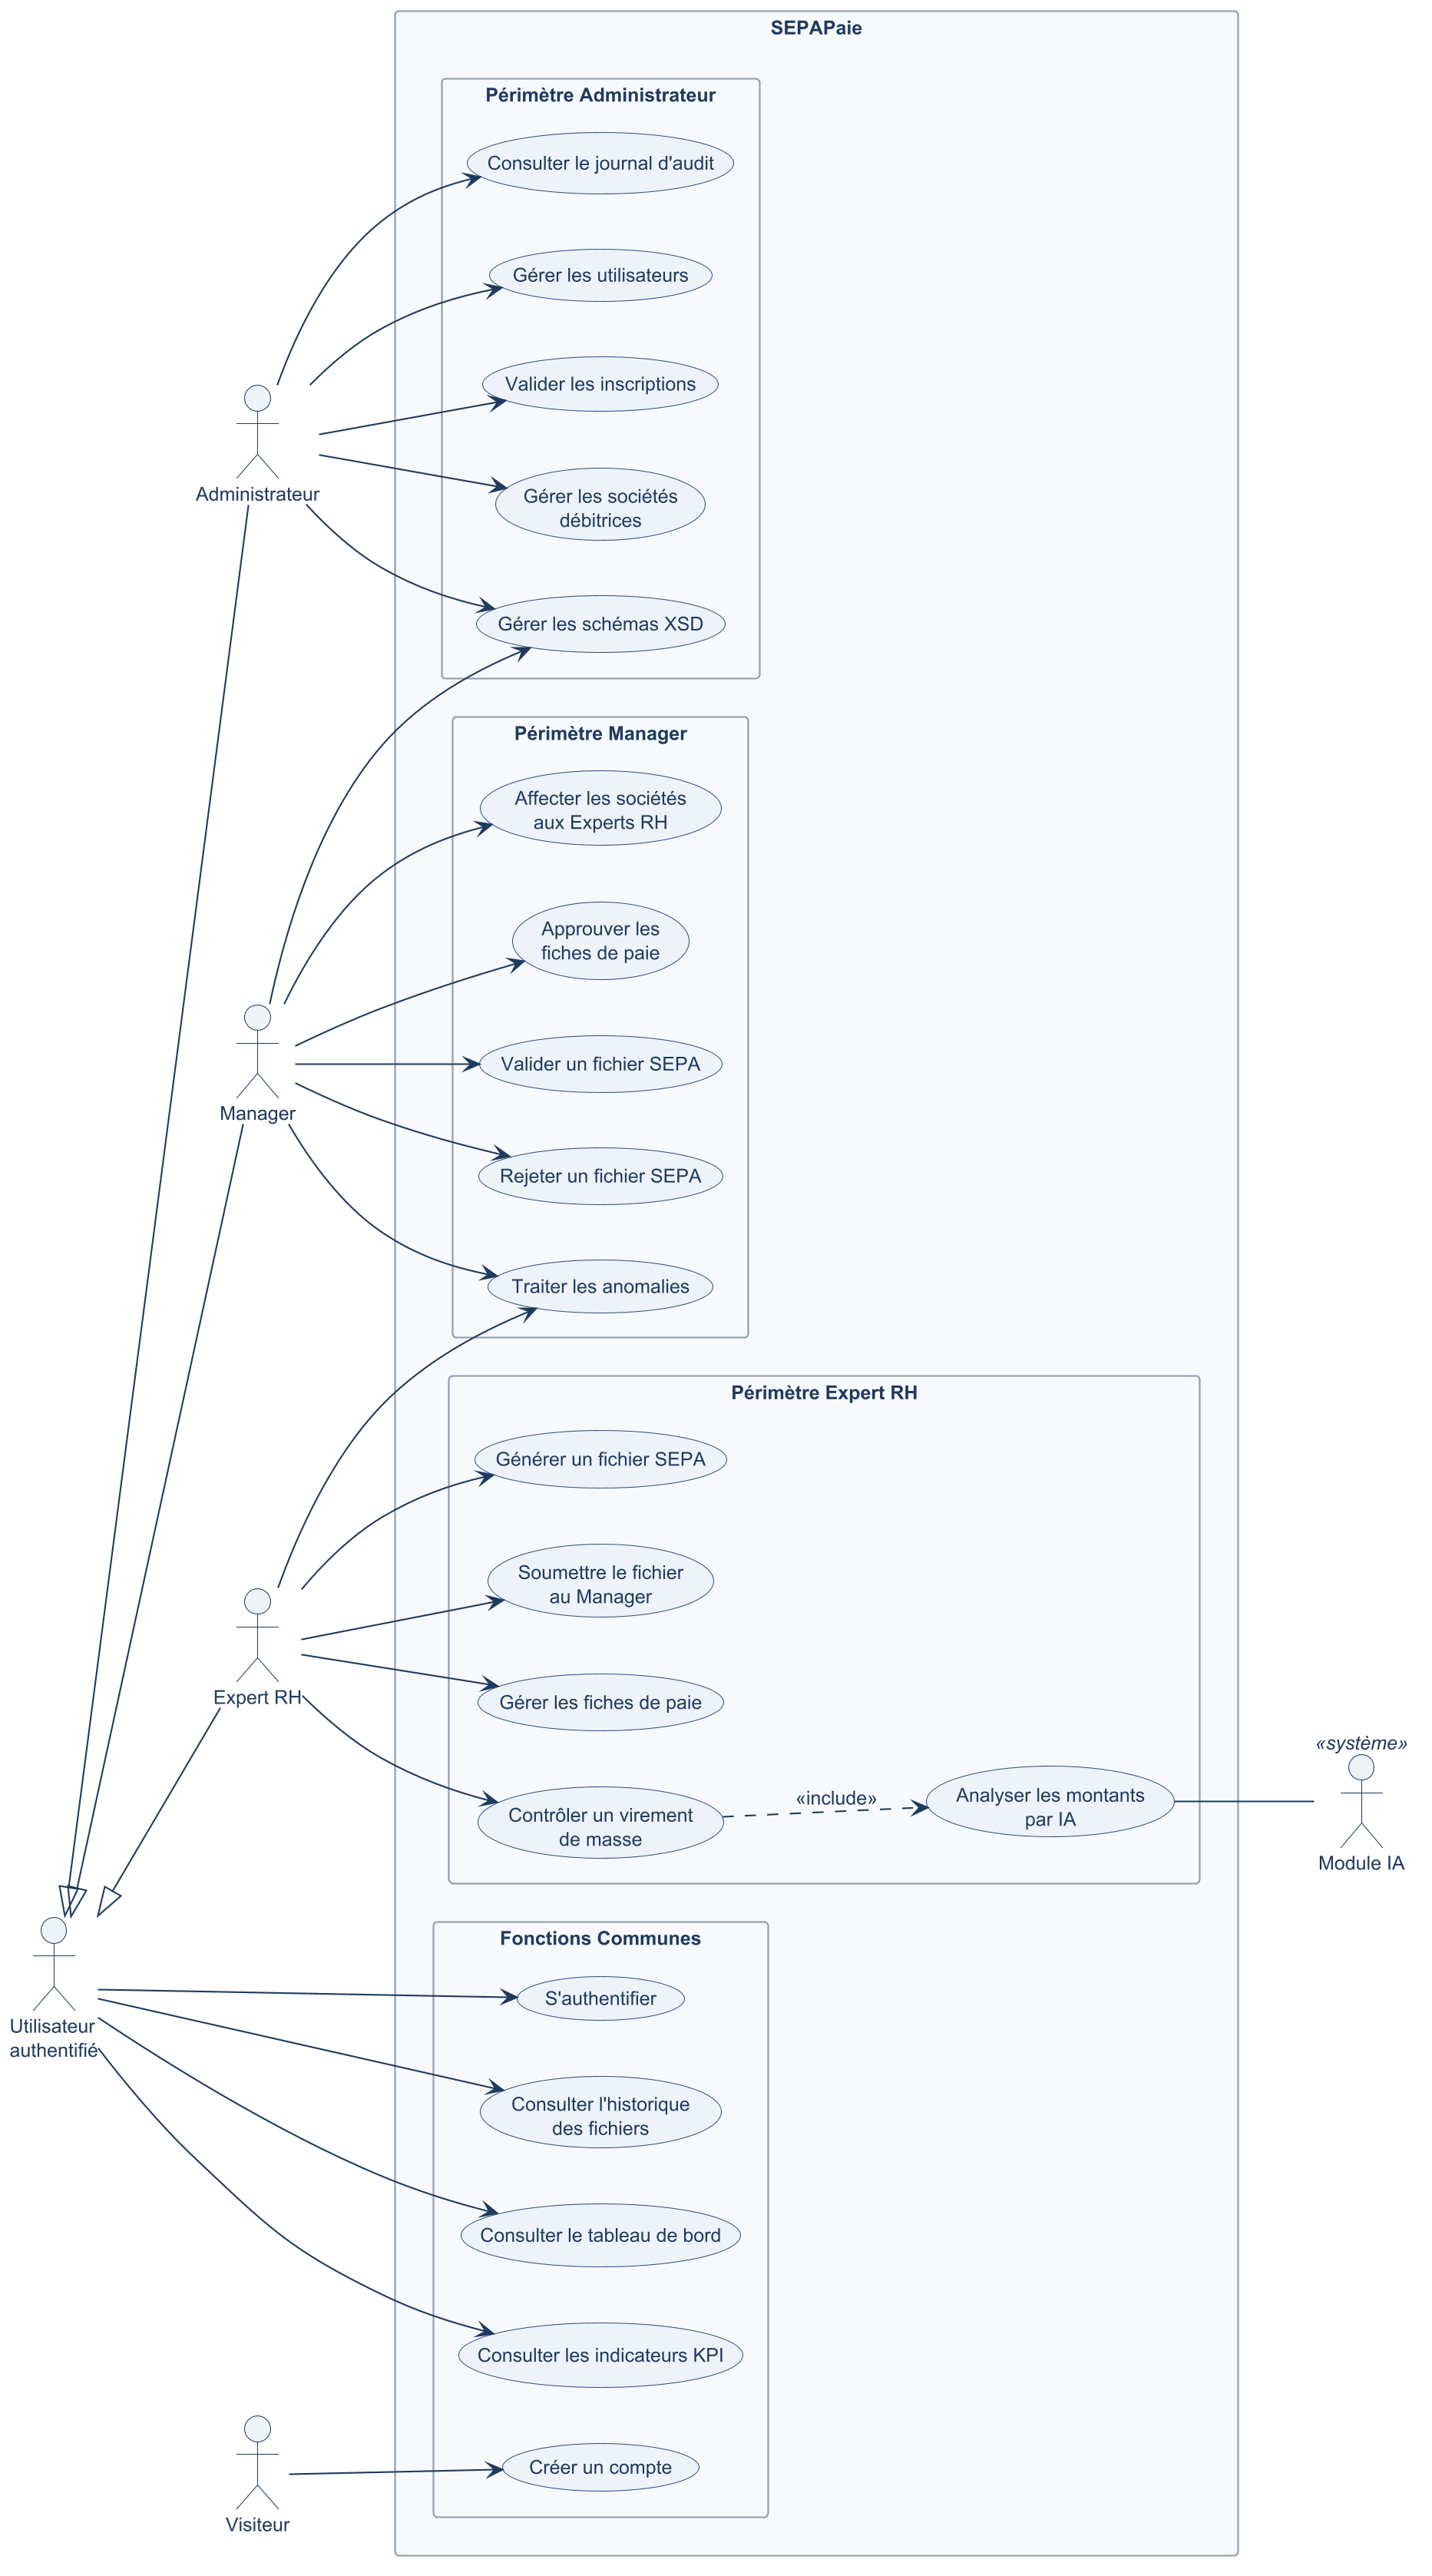
\includegraphics[height=0.78\textheight,keepaspectratio]{fig2_1_cas_utilisation_global}
    \caption{Diagramme de cas d'utilisation global}
    \label{fig:uc-global}
\end{figure}

\section{Pilotage du projet}

\subsection{Backlog produit}

Les besoins ont été traduits en récits utilisateur et priorisés avec l'encadrant professionnel. Le tableau~\ref{tab:backlog} présente le backlog produit, réparti sur les cinq sprints.

{\small
\renewcommand{\arraystretch}{1.2}
\tablestyle
\begin{longtable}{|>{\centering\arraybackslash}p{1cm}|>{\raggedright\arraybackslash}p{2.5cm}|>{\raggedright\arraybackslash}p{7.2cm}|>{\centering\arraybackslash}p{1.6cm}|>{\centering\arraybackslash}p{1.1cm}|}
\hline
\rowcolor{appMarine}\entete{N\textsuperscript{o}} & \entete{En tant que} & \entete{Je veux} & \entete{Priorité} & \entete{Sprint} \\
\hline
\endfirsthead
\hline
\rowcolor{appMarine}\entete{N\textsuperscript{o}} & \entete{En tant que} & \entete{Je veux} & \entete{Priorité} & \entete{Sprint} \\
\hline
\endhead
\endfoot
\caption{Backlog produit}\label{tab:backlog}\\
\endlastfoot
US1 & Visiteur & créer un compte avec ma photo pour demander un accès & Haute & 1 \\
\hline
US2 & Utilisateur & m'authentifier par mot de passe et code à usage unique, ou par reconnaissance faciale & Haute & 1 \\
\hline
US3 & Administrateur & valider les inscriptions et gérer les comptes et les rôles & Haute & 1 \\
\hline
US4 & Administrateur & gérer les sociétés débitrices et leurs coordonnées bancaires & Haute & 1 \\
\hline
US5 & Manager & affecter les sociétés aux Experts RH & Moyenne & 1 \\
\hline
US6 & Administrateur & consulter le journal d'audit & Moyenne & 1 \\
\hline
US7 & Expert RH & saisir des fiches de paie pour mes sociétés et les supprimer & Haute & 2 \\
\hline
US8 & Manager & approuver les fiches de paie & Haute & 2 \\
\hline
US9 & Administrateur, Manager & importer et gérer les schémas XSD & Haute & 2 \\
\hline
US10 & Expert RH & générer un fichier \texttt{pain.001} selon le schéma choisi & Haute & 2 \\
\hline
US11 & Expert RH & valider le fichier contre le XSD et en prévisualiser le contenu & Haute & 2 \\
\hline
US12 & Expert RH & contrôler un virement de masse par des règles métier & Haute & 3 \\
\hline
US13 & Expert RH, Manager & consulter et traiter les anomalies avec des recommandations & Haute & 3 \\
\hline
US14 & Expert RH & soumettre un fichier au Manager & Haute & 3 \\
\hline
US15 & Manager & valider ou rejeter un fichier soumis, avec un motif & Haute & 3 \\
\hline
US16 & Utilisateur & consulter l'historique des fichiers (en supervision pour l'administrateur) & Moyenne & 3 \\
\hline
US17 & Expert RH & être alerté des montants suspects détectés par l'IA & Haute & 4 \\
\hline
US18 & Expert RH, Manager & comprendre un signalement (explication, type probable, recommandation) & Haute & 4 \\
\hline
US19 & Équipe projet & mesurer la qualité de la détection par une évaluation rigoureuse & Haute & 4 \\
\hline
US20 & Administrateur & superviser le module d'IA et le réentraîner & Moyenne & 4 \\
\hline
US21 & Utilisateur & disposer d'un tableau de bord adapté à mon profil & Haute & 5 \\
\hline
US22 & Utilisateur & suivre des indicateurs clairement définis & Moyenne & 5 \\
\hline
US23 & Équipe technique & déployer la plateforme de façon reproductible par conteneurs & Haute & 5 \\
\hline
US24 & Développeur & disposer d'une documentation interactive de l'API & Basse & 5 \\
\hline
\end{longtable}
}

\subsection{Planification des sprints}

Le projet s'est déroulé sur sept mois, soit vingt-huit semaines. Conformément aux règles de la méthodologie Scrum, qui préconisent des itérations d'une durée maximale de quatre semaines (un mois), chaque sprint a été calibré sur une durée fixe de quatre semaines. La planification comprend une phase d'étude préalable de quatre semaines, cinq sprints de réalisation de quatre semaines chacun, et une phase de finalisation de quatre semaines. La figure~\ref{fig:gantt} en donne le calendrier, et le tableau~\ref{tab:sprints} précise l'objectif de chaque phase.

\newcommand{\gbar}[5]{%
  \node[anchor=east,align=right,font=\scriptsize] at (-0.1,-#1*0.8) {#4};
  \fill[#5,rounded corners=2pt] (#2*\w,-#1*0.8-0.25) rectangle (#3*\w,-#1*0.8+0.25);
  \node[white,font=\scriptsize] at ({0.5*(#2+#3)*\w},-#1*0.8) {\pgfmathparse{int(#3-#2)}\pgfmathresult\,sem.};}

\begin{figure}[H]
\centering
\begin{tikzpicture}
\def\w{0.41}
\foreach \m/\x in {Mars/0,Avril/4,Mai/8,Juin/12,Juillet/16,Août/20,Septembre/24} {
  \draw[appBordure] (\x*\w,0.5) -- (\x*\w,-5.7);
  \node[anchor=west,font=\scriptsize\bfseries,text=appMarine] at (\x*\w,0.75) {\m};
}
\draw[appBordure] (28*\w,0.5) -- (28*\w,-5.7);
\gbar{0}{0}{4}{Étude préalable}{grisApp}
\gbar{1}{4}{8}{Sprint 1}{appMarine}
\gbar{2}{8}{12}{Sprint 2}{appMarine}
\gbar{3}{12}{16}{Sprint 3}{appMarine}
\gbar{4}{16}{20}{Sprint 4}{appMarine}
\gbar{5}{20}{24}{Sprint 5}{appMarine}
\node[anchor=east,align=right,font=\scriptsize] at (-0.1,-4.8) {Finalisation};
\fill[acteurSysteme,rounded corners=2pt] (24*\w,-4.8-0.25) rectangle (28*\w,-4.8+0.25);
\node[white,font=\scriptsize] at ({0.5*(24+28)*\w},-4.8) {4\,sem.};
\end{tikzpicture}
\caption{Calendrier du projet (durées en semaines)}
\label{fig:gantt}
\end{figure}

\begin{table}[H]
\centering
\small
\renewcommand{\arraystretch}{1.25}
\tablestyle
\begin{tabularx}{\textwidth}{|>{\raggedright\arraybackslash}p{2.6cm}|>{\raggedright\arraybackslash}p{2.6cm}|Y|}
\hline
\rowcolor{appMarine}\entete{Phase} & \entete{Période} & \entete{Objectif} \\
\hline
Étude préalable & Mars & Étudier le domaine SEPA et ISO~20022, arrêter les choix techniques, constituer le backlog \\
\hline
Sprint 1 & Avril & Socle sécurisé : comptes, authentification, rôles, sociétés, affectations, journal d'audit \\
\hline
Sprint 2 & Mai & Fiches de paie, gestion des schémas XSD, génération et validation du fichier \texttt{pain.001} \\
\hline
Sprint 3 & Juin & Parcours de virement de masse, contrôles métier, anomalies, circuit de validation \\
\hline
Sprint 4 & Juillet & Détection par IA, intégration au parcours et évaluation du modèle \\
\hline
Sprint 5 & Août & Tableaux de bord et indicateurs, déploiement par conteneurs, recette \\
\hline
Finalisation & Septembre & Corrections finales, rédaction et remise des livrables \\
\hline
\end{tabularx}
\caption{Objectifs des sprints et des phases du projet}
\label{tab:sprints}
\end{table}

\section{Diagramme de classes d'analyse}

La figure~\ref{fig:classes} présente les principales classes du domaine, leurs attributs et leurs méthodes métier, ainsi que leurs relations. Une \textbf{société débitrice} est l'entreprise cliente dont le compte bancaire est débité : elle porte les fiches de paie et les fichiers SEPA qui la concernent, et expose des méthodes de vérification et de masquage de ses coordonnées bancaires. Un \textbf{utilisateur} est relié aux sociétés par des \textbf{affectations} datées, qui définissent le périmètre de travail d'un Expert RH. Une \textbf{fiche de paie} correspond à un virement individuel ; elle porte ses règles d'éligibilité et peut porter plusieurs \textbf{anomalies}, détectées par les règles métier ou par l'IA. Un \textbf{fichier SEPA} regroupe des fiches, respecte un \textbf{schéma XSD} et gère son cycle de vie (génération, soumission, validation ou rejet). Enfin, le \textbf{journal d'audit} conserve la trace inaltérable des actions de chaque utilisateur.

\begin{figure}[H]
    \centering
    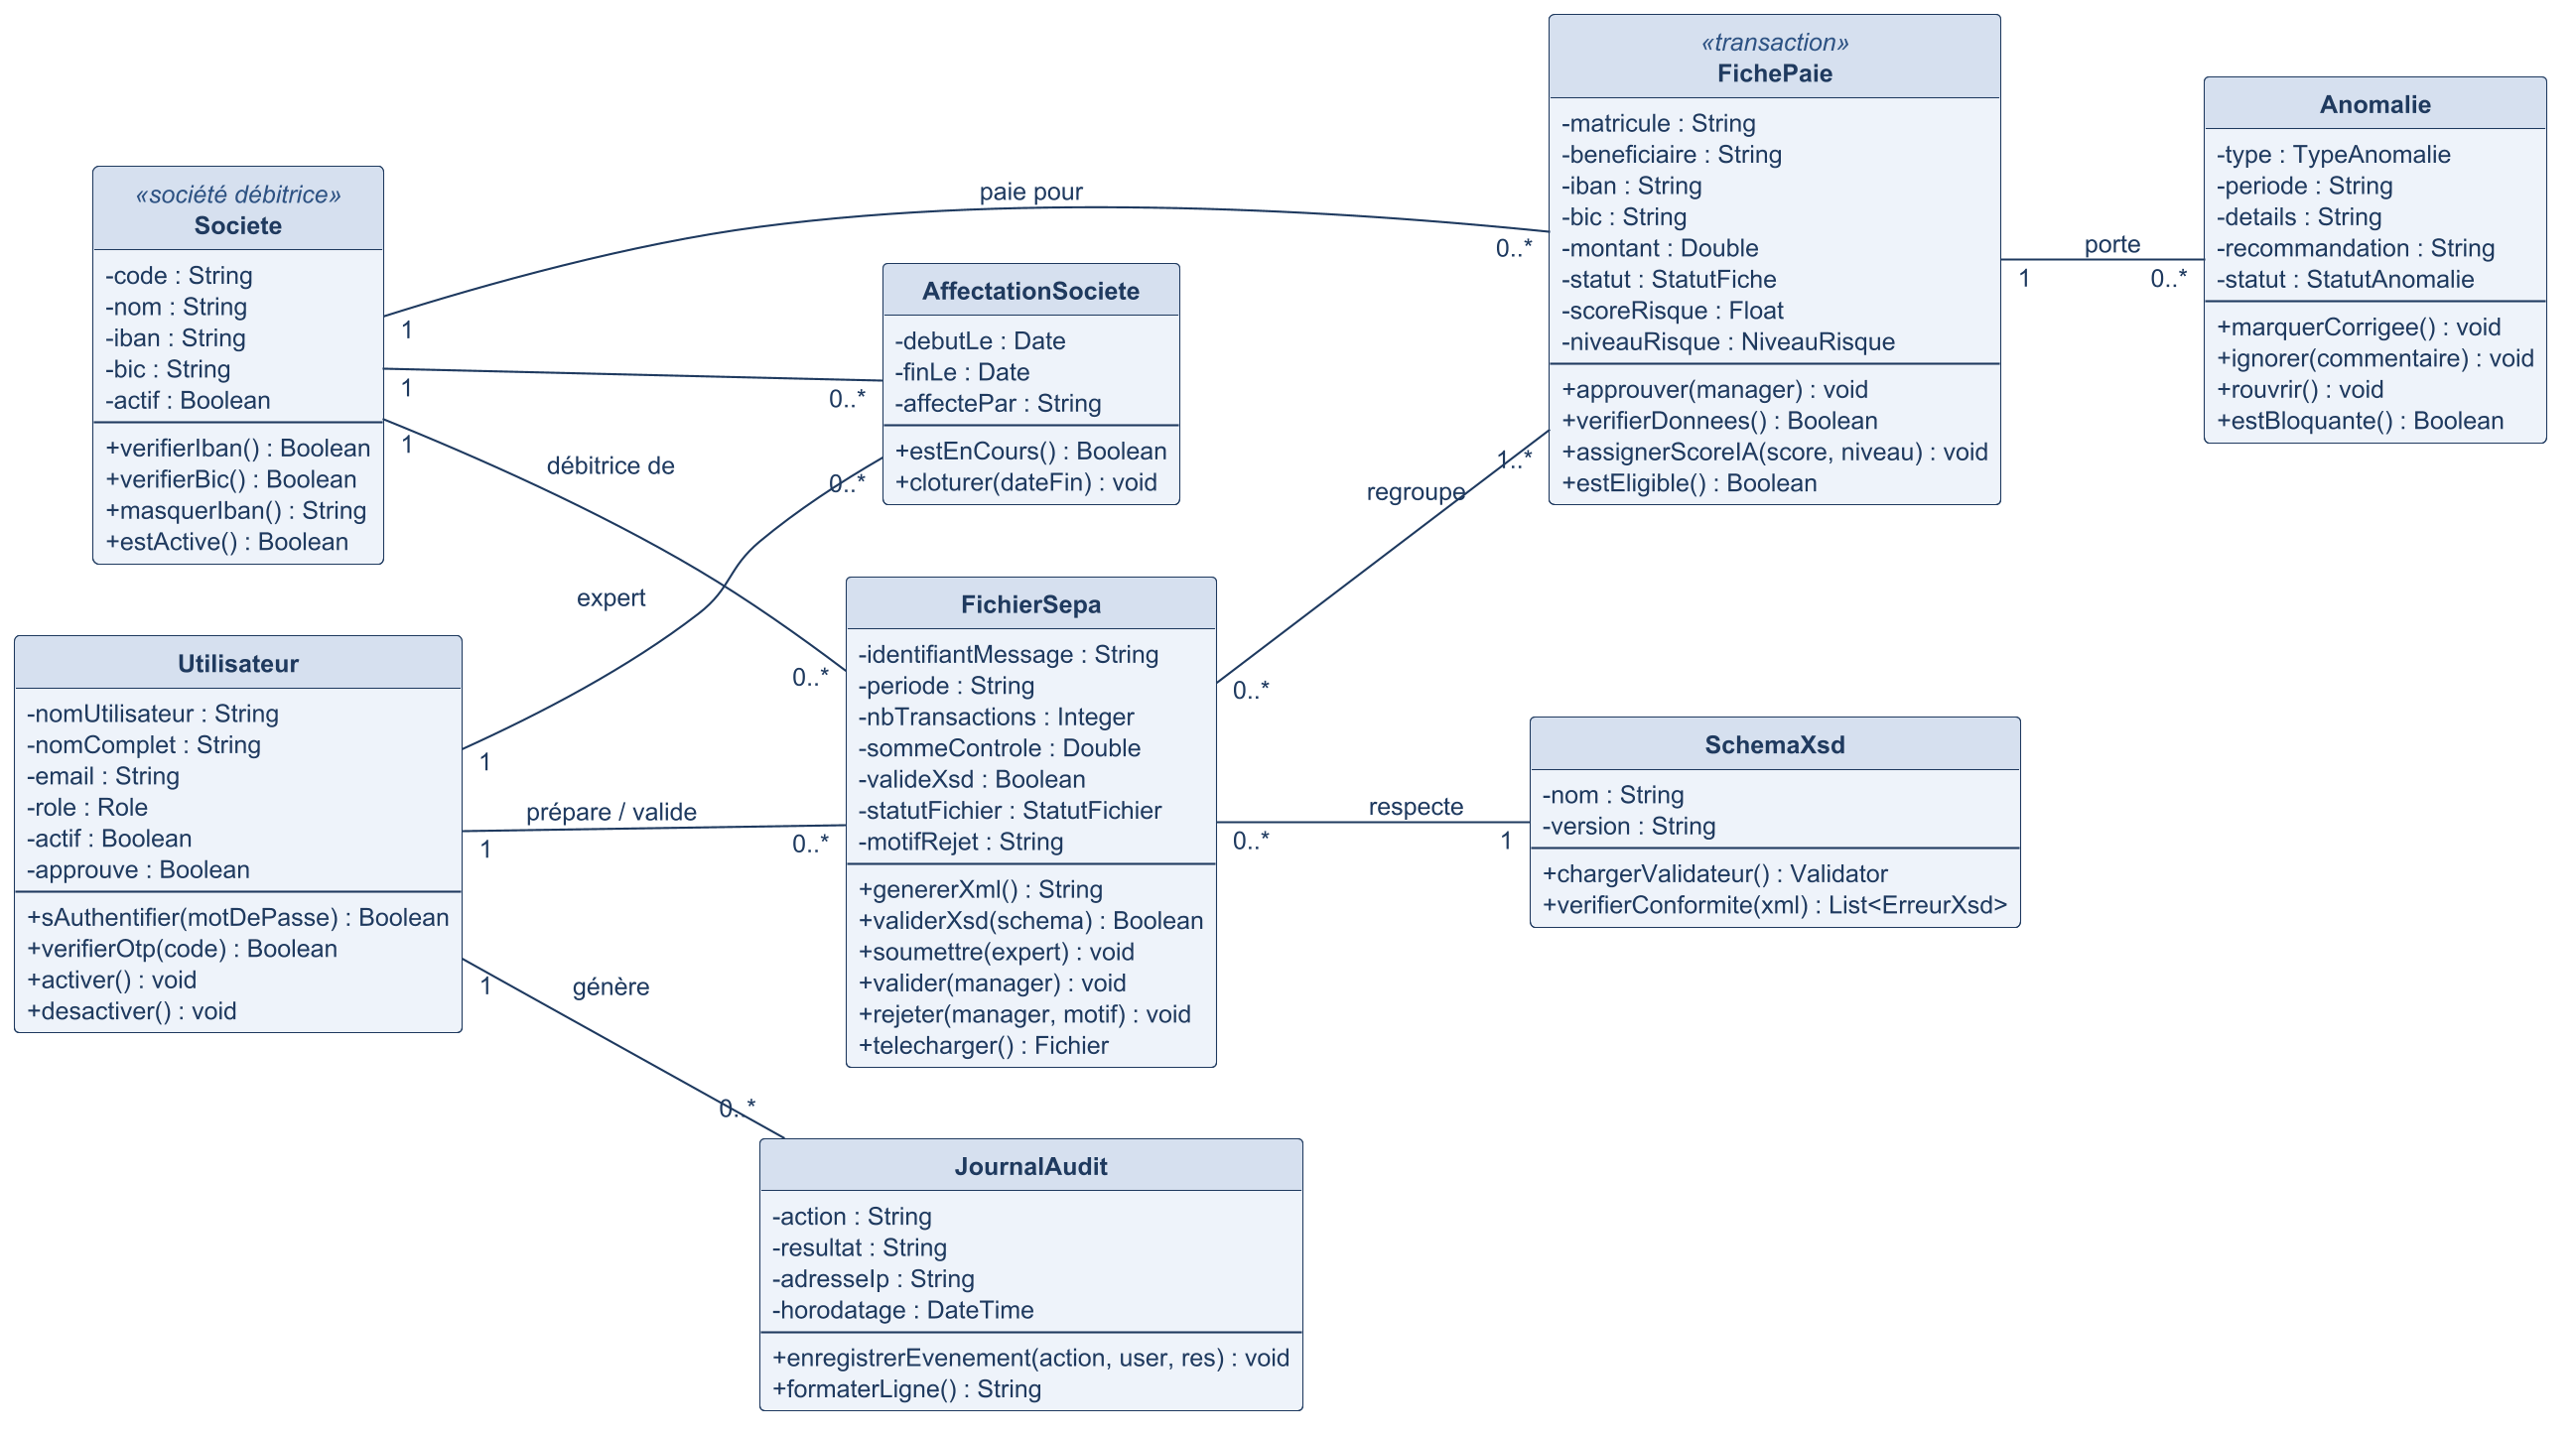
\includegraphics[width=\textwidth]{fig2_2_classes_analyse}
    \caption{Diagramme de classes d'analyse}
    \label{fig:classes}
\end{figure}

\section{Conclusion}

Ce chapitre a défini le périmètre de la plateforme : trois profils aux droits strictement séparés, sept modules fonctionnels, des exigences de sécurité, de traçabilité et d'explicabilité, et un backlog de vingt-quatre récits utilisateur. La planification en cinq sprints de quatre semaines chacun, précédés d'une phase d'étude, structure la suite de ce rapport. Le chapitre suivant présente cette étude préalable : le domaine métier, la démarche de détection d'anomalies, l'architecture retenue et les choix technologiques.

